\documentclass[conference]{IEEEtran}
\IEEEoverridecommandlockouts
% The preceding line is only needed to identify funding in the first footnote. If that is unneeded, please comment it out.
%Template version as of 6/27/2024

% \usepackage{cite}
\usepackage{amsmath,amssymb,amsfonts}
\usepackage{algorithmic}
\usepackage{graphicx}
\usepackage{textcomp}
\usepackage{xcolor}
\usepackage{capt-of}
% \usepackage[backend=bibtex]{biblatex}

\DeclareMathOperator*{\argmax}{arg\,max}
\DeclareMathOperator*{\argmin}{arg\,min}
\newcommand{\mat}[1]{\begin{bmatrix} #1 \end{bmatrix}}
\newcommand{\R}{\mathbb{R}}
\newcommand{\E}{\mathbb{E}}
\newcommand{\normal}{\mathcal{N}}

\begin{document}
\title{Predicting Lithium Ion Battery Capacity Fade under Diverse Operating Conditions Using Gaussian Process Regression}

\author{\IEEEauthorblockN{Sean Jennings}
\IEEEauthorblockA{
    \textit{Department of Electrical, Computer, and Energy Engineering} \\
    \textit{University of Colorado, Boulder, Colorado 80309}\\
    seje7952@colorado.edu}
}

\maketitle

\begin{abstract}
\end{abstract}

% \begin{IEEEkeywords}
% component, formatting, style, styling, insert.
% \end{IEEEkeywords}


\section{Introduction}

Lithium Ion batteries (LiB) have been increasingly prevalent in society since their
commericialization in the 1980s. While they appeared first in portable electronics,
the recent shift towards electrification and decarbonization has 
led to their commercialization in electric vehicles (EVs), and to a nascent, but growing degree in the power
grid \cite{noauthor_battery_2015}. 

By irreverisible electrochemical processes, the performance of
LiBs degrades over time, limiting the useful lifetime of LiB-powered devices. 
A faster degradation rate implies a shorter lifetime, and thus a greater
cost over time. Then, determining and controlling those factors correlated
with higher degradation presents an opportunity for improved economic
efficiency\cite{reniers_improving_2018} and sustainability.

While great progress has been made towards understanding the observable
mechanisms which degrade an LiB (e.g. \cite{dubarry_synthesize_2012}\cite{birkl_degradation_2017}), 
modeling degradation remains challenging due to the complex, nonlinear, and 
multiphysical nature of the process and the long time-scales involved \cite{severson_data-driven_2019}.

In this paper, we analyze an experimental LiB
dataset to gain insight into ways which LiB capacity fades under
a variety of loading conditions, with the use-case of utility-side capacity planning in mind.
We use Gaussian Process (GP) Regression (GPR) to create a
model which predicts capacity fade, a key indicator of a battery's state of health.
while taking load and stress parameters as an input. While many
authors inject information-rich signals to shed light on internal dynamics, we instead
focus on characterizing the variance over a population of battery cells.

After providing prerequisites and a mathematical formulation in the background
section, we proceed in four major steps:
\begin{enumerate}
\item validating sensor noise and removing outlying measurements,
\item examining how process noise varies over the operational space
\item using Bayesian Optimization to find length scale which maximizes likelihood of our model, and
\item showing how a "semi-emperical" model might be used as a basis within a GP kernel.
\end{enumerate}






\section{Background}

\subsection{The Use Case of LiBs within Power Systems Planning and Operations}

LiBs are increasingly being used for stationary energy storage. 
The energy transition away from carbon-burning generation sources necessitates
the integration of renewable resources such as solar and wind which are inherrently
intermittent.  To balance generation and demand amid these fluctuations, Battery Energy Storage 
Systems (BESSes) using LiBs are increasingly being integrated into the power grid \cite{noauthor_battery_2015}.

Historically, the power grid has been driving by thermal power plants fueled by coal and more recently natural gas.
Thermal power plants are considered "dispatchable" since the fuel rate can be adjusted to exactly meet demand.
Thus, only a small amount of energy storage was necessary. Stationary grid storage applications
are expected to grow substantially as more renewables are integrated,
with BESSes accounting for a substantial portion. 

CEMs have been used for many years by power system planners to determine the most efficient allocation of capital investments. CEMs are tied to a production cost model (PCM) which accounts for the variable operational costs of running particular generators. CEMs solve an optimization problem, which can be roughly phrased: which generators and transmission
lines should be constructed to minimize costs under the constraint that generation meets projected demand.
Since energy infrasture involves large upfront capital investments, there is a strong incentive to build high fidelity models
to inform the decision-making process.

Since BESSes have never been integrated into the power grid on a large scale, they represent a new frontier in capacity expansion modeling.
While there exists a significant body of research which investigates how to optimally size batteries within a power system, to the extent of the author's knowledge,
they make very simplistic assumptions about the lifetime of BESSes. Many assume either that 1) the lifetime of BESSes are fixed period, or 2)
(what's the other assumption???). 

As we shall see in the following section, capacity fade of LiBs is a complex phenomenon. This motivates the main topic of this paper:
a capacity fade model which is appropriate for system-level CEMs.

\subsection{Degradation Mechanics of LiBs}

\subsubsection{Battery Basics}

A galvanic cell (referred to as just "cell" for the remainder of the paper)
is a basic unit of energy storage which enables electrical energy
to be stored in a chemical form for some length of time, for later use.
Figure [] alongside a conceptual model of its major components.

When the terminals
of the battery are connected by an electrically conductive material, a closed circuit
is formed. Inside the cell, positive ions flow from the high energy
positive electrode PE (or cathode), to the lower energy negative electrode (NE)
(or anode), via an electrolyte. An oxidation reaction (loss of an electron) occurs at the PE
while a reduction reaction (gain of an electron) occurs at the NE. The oxidation
reaction releases more energy than the reduction reaction requires, thus
generating energy in the form of a moving electron.

In a rechargeable cell, when an electrical potential is applied to
the terminal, along with a flow of electrons, the positive ions flow
in the opposite direction, towards the PE, where they remain at a 
higher energy level.

LiBs are one family of battery chemistries where the positive ion
is Lithium. They have a number of advantages over other battery
chemistries, including rechargeability, a long lifetime, and high
energy/power density.

There are numerous physical phenomenon which occur inside an LiB cell,
including chemical reaction kinetics, diffusion within the electrodes,
and electrostatic-driven flow through the liquid electrolyte.

The Doyle, Fuller, and Newman (DFN) model \cite{doyle_modeling_1993} laid the foundation
for electrochemical modeling of LiBs, proposing a governing set of
partial differential equations, from which many subsequent symmetry-utilizing
model reductions have been derived. This electrochemical modeling
is the tool of choice when a high fidelity simulation of an LiB
is desired. 

But electrical engineers who integrate LiBs into larger systems
typically desire a lower order model which captures a LiB's input-output
behavior in terms of an algebraic relationship between voltage and current.
To this effect, numerous equivalent electrical models (ECMs) and
impedance-based models have been proposed. Figure \ref{fig:ecm} adapts the
ECM proposed by \cite{chen_accurate_2006}, which we find to be illustrative
as well as suitable for our use case because it accomodates a time-vary capacity.
We use this ECM for conceptual purposes, adopting a more mathematical
and less circuit-simulator-specific interpretation.

Figure \ref{fig:ecm}a shows the capacity-related side of the equation: a
capacitor which can store a maximum of $c(t)$ charge (e.g. measured in Ah).
It is connected with a current-controlled source, which is algebraically
equivalent to the current flowing through the circuit of Figure \ref{fig:ecm}b.

Let $q(t)$ denote the state of charge (SoC) which is a dimensionless
quantity between 0 and 1, where a value of 0 denotes that the battery
is fully discharged, and a value of 1 indicates that the maximum charge 
$c(t)$ is stored. The current $I(t)$ and SoC are
related by the expression:

\begin{align*}
    I(t) = \dot{q}(t) c(t)
\end{align*}

The capacity $c(t)$ is not directly observable, but can be accurately
inferred by executing a full charge/discharge cycle.

The current source of Figure \ref{fig:ecm}(a) is algebraically equivalent to the
the current flowing through the circuit in Figure \ref{fig:ecm}(b), which is
determined by the series combination of a voltage-controller source
$v_{oc}(t) = OCV(q(t))$ depedent on the SoC, a resistor $R_e$ coupled with an RC
pair $R_{qt}$ and $C_{dl}$, and finally a load.

A typical OCV curve is depicted in Figure \ref{fig:ecm}(c). The components $R_e$, $R_{qt}$ and $C_{dl}$
provide a time-domain representation of the internal impedance of the battery. We
label them in correspondence with their electrochemical origins. $R_e$ denotes
the resistance of the electrolyte, which responds at the fastest timescales, while
$R_{qt}$ denotes the resistance associated with the charge transfer kinetics occurring
at the electrode surfaces. $C_{dl}$ refers to the "double layer" capacitance, which is
the physical phenomenon in which a capacitive layer of charge forms along the electrode
surfaces.

\begin{center}
    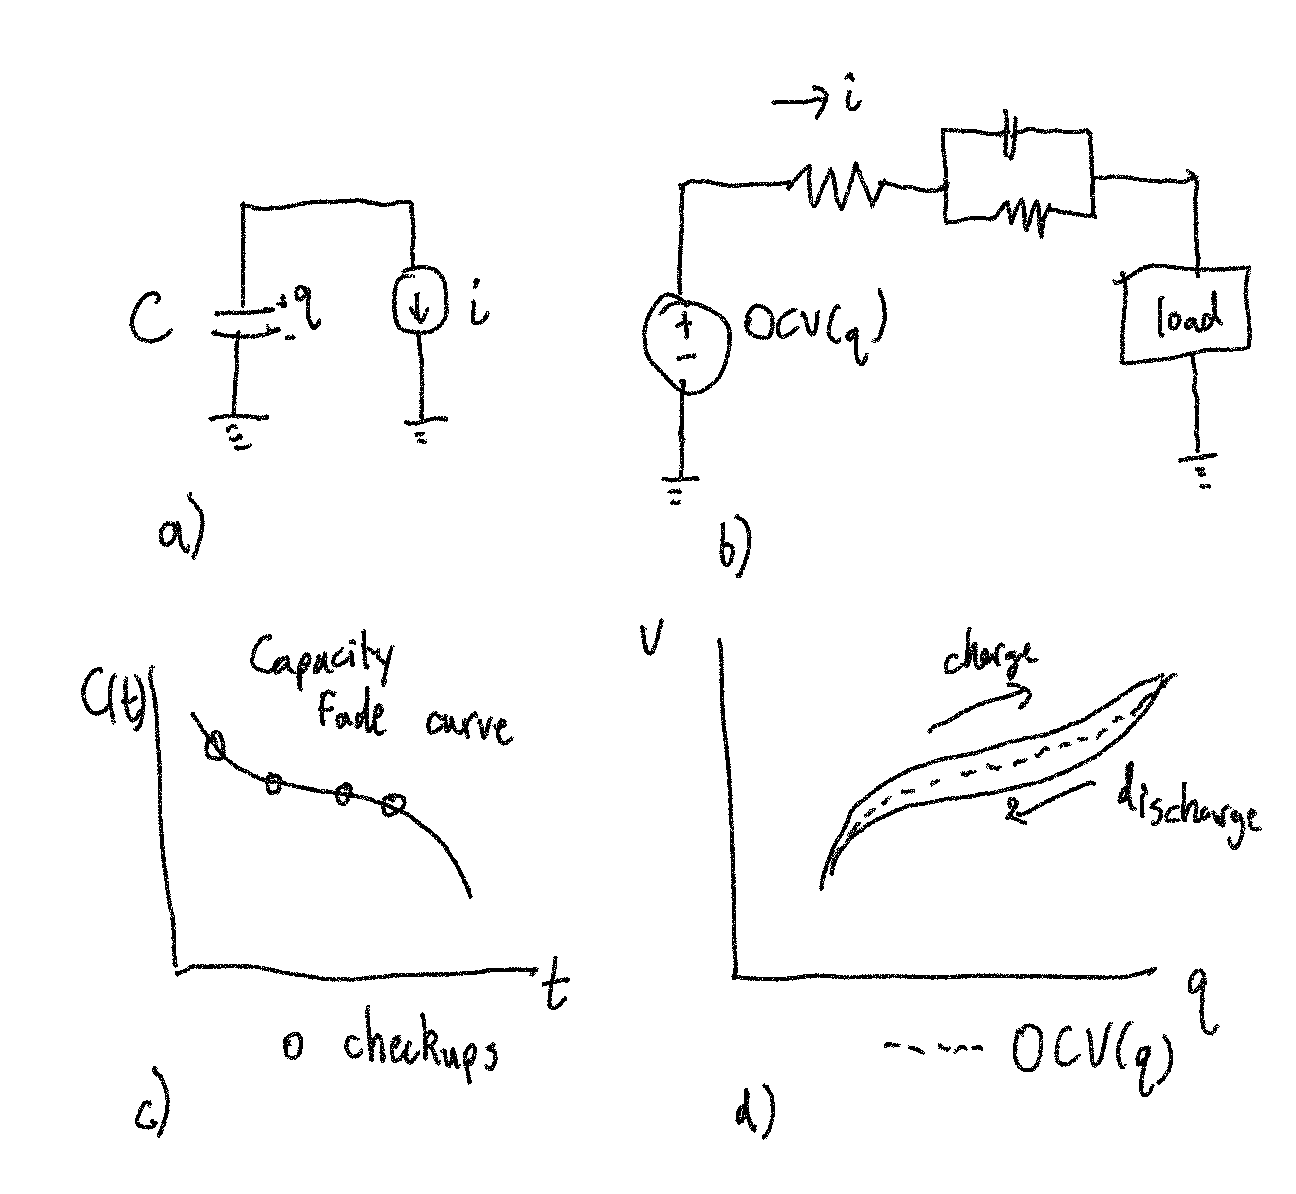
\includegraphics[width=0.8\linewidth]{Images/ECM.png}
    \captionof{figure}{Second-order Equivalent Circuit Model (ECM)}
    \label{fig:ecm}
\end{center}


The correspondence between ECMs and the true electrochemisty-based physics is perhaps best
understood through a Nyquist plot, which plots the frequency response $Z(\omega)$ as a curve
on the imaginary plane. A Nyquist plot for a typical LiB is shown in Figure [].
The bottom-most portion of the semi-circle in the lower half plane is the response
at high frequencies (>1 kHz), and shows inductive behavior (current lags voltage).
The response is purely resistive around 1kHz, corresponding to electrolyte-related
resistance. The portion of the semi-circle in the upper half plane corresponds to
capacitive dynamics occurring at the electrode surface. Finally, the low frequency
tail ascending into the upper right half plane at a 45-degree angle corresponds 
to diffusion within the electrode (this can be modeled by the non-physical Warburg impedance element)

While some authors view ECMs and impedance-based models as distinct \cite{seaman_survey_2014}, we argue they
can be viewed as dual representation of a single object. Impedance-based models are samples
of the system transfer function, and linear system theory demonstrates that any 
transfer function that is a proper rational function has a state-space realization, from which
an ECM can be derived.
representation of the system transfer function, and linear system theory shows that
there

% We note that the frequency response is primarily a 



% high frequency
% A Nyquist plot of a typical LiB is shown in figure [].




 This current source is connected to be algebraically
equivalent to the current passing through the voltage source on the right
hand circuit. Simultaneously, the voltage at the voltage source is a
function $OCV$ of $q(t)$, diplayed in figure \ref{fig:ecm}(d). Note that the voltage
varies rapidly as SOC approaches its maximum and minimum: this is 
a result of charge saturation in the PE and NE, respectively.

In a slight abuse of notation, we write $q(t)$ (since the symbol $q$
is typically reserved for a charge with dimension of Colombs),
as a dimensionless
parameter taking values between 0 and 1. If $\bar{q}(t)$ is the charge
at the capacitor, then
\begin{equation*}
    q(t) = \frac{\bar{q}(t)}{c(t)}
\end{equation*}
where $c(t)$ is the total capacity measured in Ah.




The state of charge (SoC) $q(t)$ is the a dimensionless
state variable taking values between 0 and 1, which models the amount of charge
available within the battery, with 1 corresponding to a full charge, and
0 to total depletion, as attained by a constant current, constant voltage (CCCV)
charge profile.

The State of Health (SoH) is a multi-faceted attribute of a battery which encapsulates
how well it is able to perform compared to its original, nominal state.
Measureable symptoms of a declining SoH are:
\begin{itemize}
    \item capacity fade -- the batteries ability to hold charge decreases over time
    \item power fade -- the battery is unable to output maximum power as it ages
    \item increased internal resistance -- as the cell ages, charge flows less efficiently,
        and more heat is generated.
\end{itemize}


Another important metric is remaining useful life (RUL) is typically
defined in terms of capacity fade.

Let $c_0$ be the initial, nominal
capacity of a cell and $c(t)$ is its capacity over time.
Let $i(t)$ be the current that leaves the cell at time $t$
and $q_+(t)$ be the total amount of discharge over the lifetime of
the cell. Specifically,
\begin{equation*}
    q_+(t) = \int_{t_0}^{t} i_+(t) dt
\end{equation*}
where $t_0$ is the time of cell manufacture and $i_+$ is given by
\begin{equation*}
    i_+(t) = \biggl\{
        \begin{array}{ll}
            i(t) &\quad \text{if } i(t) >= 0 \\
            0 & \quad \text{otherwise.}
        \end{array}
    \biggr.
\end{equation*}

We then define the number of "full equivalent cycles" (FEC) $k(t)$ at time $t$
to be the number of complete charge/discharge cycles performed up to
time $t$.  This is expressed as $k(t) = q(t) / c_0$.
%     \footnote{
%     Note that this is defined in terms of current, while really
%     the metric of interest should be energy-over-lifetime.
%     In the case of periodic cycling, total energy of the curve
%     depends on the the product of voltage and current.
% }



The end of life of an LiB is typically defined in literature
as the time $t_f$ at which the capacity has reduced to some
predefined capacity $c_f$. Mathematically,
\begin{equation*}
    t_f = \argmin_t \{t | c(t) = c_f\}   
\end{equation*}

Finally, we can define the RUL $r(t)$ as the remaining number of FECs:
\begin{equation*}
    r(t) = k(t_f) - k(t)
\end{equation*}

In literature, $c_f$ is commonly taken to be 80\% of the nominal
capacity, i.e. $c_f = 0.8 c_0$.  It is unclear to the author the exact
source of this common 80\% assumption, but it seems to have origins
in the EV space, where capacity fade corresponds to a reduction in
the range of the vehicle and 80\% range is the point at which performance
is deemed unacceptable. Whether this assumption is pertinent
in a stationary energy storage setting is questionable (e.g. in the
context of second-life battery usage). We therefore seek to parameterize
the capacity fade curve, from which the RUL can be determined as 
a function of $c_f$ and the loading curve $k(t)$.

There are multitude of mechanisms by which degradation occurs, many
of which depend on the specific chemistries in question.
But in general, they pertain to the micro- and macro-scale changes to the solid electrolyte
interface (SEI), at which Lithium ions are exchanged via a chemical redox
reaction. The degradation rate is typically higher at the start of a cell's
life because an inert layer forms on the SEI, consuming the inventory of
lithium.  The repeated "intercalcation" of ions into the solid structure
of the electrode, over time causes stress fractures and structural damage to
the electrode. Newly exposed surface must form a new SEI layer, causing further
loss of lithium inventory (LLI). The active material of the electrode
refers to sites that are able to accept Lithium ions. The Loss of active material
(LAM) is another source of capacity fade.

These mechanisms (LLI and LAM) are observable from the Open Circuit Voltage
(OCV) curve of a LiB cell. In fact, the change in the OCV over time
is shown to be highly correlated with RUL [Severson, et al].

Electrochemical Impedance Spectroscopy (EIS) is another method which
is reveal rich information about the internal dynamics of 
an LiB cell, by injecting low-amplitude signals across a wide spectrum
of frequencies, and observing the impedance response. Zhang et al.
recently shows that the a model trained on EIS can accurately predict
RUL and that impedance response around 15 Hz was the feature more highly
correlated with RUL. This frequency range is associated
with charge transfer at the electrode, which corroborates the
assumption in mechanistic models that degradation mainly results from
changes at the SEI.

\subsubsection{Stress factors which affect degradation}

The degradation rate of LiBs also depends heavily on the conditions
in which the cell operates. The core temperature internal to the LiB
cell directly impacts the rates of degradation-related chemical reactions:
generally, higher operating temperatures lead to faster aging rates.
Via the laws of heat transfer, the core temperature $T_c$ is related to
the ambient temperature $T$ via convective heating/cooling and to the
(dis)charge rate (C-rate) which generates heat due to resistive
losses.

The specific shape of the charge curve also affects aging in more
complex ways, governed by the set
partial differential equations defining electrochemical dynamics.
For instance, SEI growth is related to
the overpotential at electrodes and advanced battery management systems
(BMS's) can model the constraints posed by these dynamics to
operate in space which more optimally balances the trade-off between
maximizing C-rates and minizing aging.

However, the inherent high-dimensionality of such detailed modeling
can be computationally burdensome for the power system models discussed
in the subsequent section. Therefore, we seek reduced-order models
which can accurately predict the aging process when the load
profile is restricted to some manifold of the full operations
space. Examples of such restrictions include constant current-constant
voltage (CCCV) profiles, constant current (CC) profiles, or the
more advanced moving boundary profiles described in [].




\subsection{Gaussian Processes}

\subsubsection{History and Intuition}

Gaussian Processes Regression (GPR) is today a technique commonly used
within the broad Machine Learning community, and more specifically
within battery estimation literature. GPs have the major advantage of
handling of uncertainty methodically, owing to its rigourous
mathematical foundation with roots in the
theory of stochastic processes, developed by Komolgorov in the 1930s.
GPR was by the pioneering work of Rasmussen and Williams in the
1990s. Their book "Gaussian Processes for Machine Learning" is a canonical
introduction to the subject.

Interestingly, there is a direct correspondence between GP and the method widely known
as Kriging within the geostatistics community. Essentially, GPs extend Kriging
into a Bayesian framework. Under the assumption that distribution of any finite set
of points in a random field is jointly Gaussian, the Best Linear Unbiased
Estimator (BLUE) for which the Kriging System solves corresponds to the
Maximum A Posteriori (MAP) estimator of a GP. The mean square error in
the BLUE is equivalent with the variance of the GP.
See \cite{marinescu_explaining_2024} for a complete treatment.


The author finds that Kriging within a geophysical context serves as a useful tool
for intuitively visualizing how GP Regression works. Generating a surface map
of the earth's topology by smoothly interpolating between a sparse sampling of altitude
measurements or guessing the best place to mine for gold based off drilling core samples
is perhaps not that different from state of the art LiB SoH estimation
techniques.

Of course, this is not to downplay the important fact that each of these physical
examples has unique properties, defined by the underlying physical nature
of the system to be estimated. Within the context of GPR, the selection of an appropriate
covariance function, or kernel serves the purpose of capturing these known properties.

\subsubsection{Formal Definition}
\label{sec:gp}

\newcommand{\X}{\mathcal{X}}

We define a Gaussian process to be a collection of real random variables
$f(x)$ associated with a space $\R^N$, any finite subset of 
which are jointly Gaussian. It is fully defined by its mean
function $m(x): \R^N \to \R$ and its covariance function
$k(x, x'); \R^N \times \R^N \to \R$ by the relations:
\begin{align*}
    m(x) &= \E[f(x)] \\
    k(x, x') &= \E[(f(x) - m(x))(f(x') - m(x'))]
\end{align*}

The covariance function is analogous to the variogram of a Kriging
filter and defines how closely correlated points $x$ and $x'$ are,
typically based on the distance between them.

Using Rasmussen's notation, we write
$K(X, X'): \R^{M\times N} \times \R^{P\times N} \to \R^{M\times P}$
to indicate the covariance between each pair of a set $X$
consisting of $M$ points and a set $X'$ of $P$ points. 
Specifically, if 
$y_i = f(x_i)$, then the $ij$th entry of $K(X, X')$ is given by:

\begin{equation*}
    \label{eq:covariance-def}
    \text{cov}(y_i, y_j) = (K(X, X))_{ij} = k(x_i, x_j)  \\
\end{equation*}
for $i=1,\dots M$ and $j=1,\dots P$.

We now pose the problem of predicting the value of $y_i^*=f(x_i^*)$
at a set of $P$ prediction points $x_i^*\in\R^N$, based on the
a set of $M$ observations $Y\in\R^M$ associated with
points $X\in\R^{M\times N}$.
By the definition of the Gaussian processes, we assume these
draw from the joint distribution
\begin{equation*}
    \mat{Y \\ Y^*} \sim \normal\biggl(0, \mat{
        K(X, X) & K(X, X^*) \\
        K(X^*, X) & K(X^*, X^*) \\
    }\biggr)
\end{equation*}

To estimate $Y^*$ we can use Bayes' rule to compute the posterior
distribution:
\begin{equation} \label{eq:posterior-dist}
    Y^* | X^*, X, Y \sim \normal(\mu, \Sigma)  
\end{equation}
where $\mu\in\R^P$ is the mean of the posterior distribution, given by
\begin{equation*} \label{eq:mu}
    \mu = K(X^*, X) K(X, X)^{-1} y,
\end{equation*}
and $\sigma\in \R^{P\times P}$ is the covariance of the posterior
distribution, given by
\begin{equation*}
    \Sigma = K(X^*, X^*) - K(X^*,  X), K(X, X)^{-1} K(X, X^*).
\end{equation*}
A proof of this explicit formula of the conditional distribution 
can be found in \cite{williams_gaussian_2006}(Appendix A2).

Note that the mean of this distribution corresponds to the
fundamental result of estimation theory, discussed in lecture:
that the optimal linear estimator 
\begin{align*}
    \hat{x} = D y
\end{align*}
is given by
\begin{equation*}
    D = R_{xy} R_{yy}^{-1}.
\end{equation*}

To see the correspondence, put the lecture's $y$ as
$Y = f(X)$ and the lecture's $x$ as $Y^* = f(X^*)$.
Then, $R_{xy}$ corresponds to $\text{cov}(Y, Y^*) = K(X, X)$
and $R_{yy}$ to $\text{cov}(Y^*, Y^*)$ by equation
(\ref{eq:covariance-def}). The key difference is that
the viewpoint in lecture makes the underlying process $f$
implicit. (At least in terms of the presentation of Kriging;
of course, explicit process models were used elsewhere
in the course.)

\newcommand{\norm}[1]{\lVert #1 \rVert}
The most common kernel function used for a Gaussian process is
the squared exponential (SE), given by:
\begin{equation*}
    k(x, x') = \sigma^2 \exp\biggl(\frac{\norm{x - x'}^2}{2 \ell}\biggr)
\end{equation*}

where $\sigma$ is the process noise and $\ell$ is the length
scale, and collectively they are referred to as the
hyperparameters of the kernel, $\theta$. In this case,
$\theta=[\sigma, \ell]^T$.

The left-multiplication by $K(X*, X)$ in equation \ref{eq:mu}
means that prediction points $x^*$ are more heavily
weighted by measurements $y_i=f(x_i)$ taken at nearby points,
where $\norm{x^* - x_i}$ is small.

It is common to perform "Bayesian model selection," which finds
the hyperparameter with the greatest likelihood. That is,
we want to find its posterior distribution:
% the marginal probability $p(\theta |y,X)$ over the
% hyper-parameters $\theta$.  That is,
\begin{equation*}
    \label{eq:model-select}
    p(\theta | y, X) = \frac{p(y|X,\theta)p(\theta|X)}{p(y|X)}
\end{equation*}
where $p(y|X)$ is the marginal likelihood, over $\theta$
\begin{equation*}
    p(y|X) = \int p(y|\theta, X) p(\theta) d\theta.
\end{equation*}

where $p(\theta)$ is the prior for the hyperparameters.




\section{Methods}

\subsection{Experimental Dataset and Preprocessing}
\label{sec:dataset-proc}

While many LiB aging datasets exist, we opt to investigate
the data generated from the experiment by Stroebl, et
al.\cite{stroebl_multi-stage_2024} because
it varies the greatest number of stress factors and the portion of the
operating space that it explores is well tailored to stationary storage
applications. 

In this experiment, each of 227 distinct LiB cell (Samsung INR21700-50E)
undergo a test protocol. The cells are divided into two groups:
one which undergoes calendar aging and the other, cycle aging.
We restrict our attention to the $P=140$ cells which constitute the cycle
aging group.

Each test alternates between checkups and cycling periods.
During each checkup, two capacity measurements are taken via a
CCCV charge profile and a CCCV discharge profile, among other tests
(i.e. OCV and hybrid power pulse characterization). 
During cycling periods, the cell is cycled according to the operational
parameters $u$ described in section [].

Given the high-dimensionality of the operation space $\mathcal{U}$,
the experimental set $\mathcal{U}_E$ =$\{u_i | i \in [1, \dots P]\} \subset \mathcal{U}$
is selected via design of experiment techniques in two stages,
the first using a Latin hypercube design and the second a parameter optimal
individual experimental design.

The dataset is stored in a ZIP file which consists of:
\begin{enumerate}
    \item the file {\it experiments\_meta.csv},
    each row of which documents the operating conditions $u_i$ for a particular
    LiB cell,
    \item a series subdirectories, each corresponding to an individual cell,
    which in turn contain a series of {\it csv} files 
    consisting of voltage, current, and temperature measurements
    taken during each step of the experiment.
\end{enumerate}

We write Python code which iterates through each folder in the directory
structure and extracts the features of interest:
\begin{enumerate}
    \item the capacity measurement $c_{mn}$ at checkup $m$
        ($m=1,\cdots M_i$, $n\in[1, 2]$), and
    \item the number of FECs $\Delta k_m$ ($m=1,\dots, M_i - 1$) occurring
        between checkup $m$ and $m+1$,
\end{enumerate}

where $M_i$ is the total number of checkups performed on cell $i$,
$n=1$ corresponds to the capacity measured by discharge CCCV and $n=2$
the second measurement by charge CCCV. We note that the additional "cycles"
associated with the discharging during checkups are neglected. We leverage
the code provided by the dataset authors for feature extraction.

The total number of FECs $k_m$ at checkup $m$ is computed from
$\Delta k_m$ via a cumulative sum:
\begin{equation*}
    k_1 = 0, \quad k_{i} = k_{i-1} + \Delta k_{i-1} \qquad (i=2,\dots M_i).
\end{equation*}

We finally aggregate the results across all cells into a matrix $X\in\R^{M\times N}$
with row $j$ given by:
\begin{align*}
    x_j = \mat{
        u_i^T & \hat{T}_m & k_m
    } \\ i\in[1,\dots P], m\in[1,\dots,M_i]
\end{align*}
and a vector $y\in\R^M$ with its $j$-th entry given
by the average capacity during charge and discharge at each of
the $M$ checkups.
\begin{equation*}
    y_j = \frac{c_{m1} + c_{m2}}{2}
\end{equation*}

The number of rows, $M$, of matrix $X$ corresponds to the 
total number of checkups across all cells, i.e. $M = \sum_{i=1}^{P} M_i$.

We will refer to the number of columns, $N$, of $X$ to be the 
number of features. $N=7$ for the full dataset.

$\hat{T}_m$ represents the measurement temperature (which may be distinct
from the temperature during cycling, particularly during initial and final checkups).

$u_i$ is the operating conditions of cell $i$
\begin{equation*}
    u_i = \mat{Q_i & \Delta_i & \gamma_{d,i} & \gamma_{c,i} & T_i}
\end{equation*}
The operating conditions are equivalent to the ones which are varied
by Stroebl et al. We use the notation $Q$ to indicate the max SoC
during cycling, $\Delta$ to denote the depth of discharge (fraction of
the whole capacity used per cycle), $\gamma_d$ and $\gamma_c$ indicate
the discharge and charge currents, respectively, and $T$ denotes the ambient
temperature during cycling. 
Figure [] gives a graphic description of this CC charge/discharge profile.

% Following the lead of Stroebl et al., we restrict our attention
% to CC curves which can be parametrized as a periodic SoC profile
% $q_u(\tau)$ which depends on the a given set of stress parameters $u$:

% \begin{equation*}
%     q_u(\tau) = \biggl\{
%         \begin{array}{ll}
%             Q - \gamma_d \tau  &\quad \text{if } \tau \in [\tau_0, \tau_0 + \tau_d] \\
%             Q - \gamma_d \tau_d + \gamma_c(\tau - \tau_c) &\quad \text{if }\tau_0\in [\tau_0 + \tau_d, \tau_0 + \tau_d + \tau_c]
%         \end{array}
%     \biggr.
% \end{equation*}

% where $Q$ represents the max SoC, $\gamma_d$ 

\subsection{Estimating Capacity Measurement Noise}
As described in section [], the capacity $c$ is defined as the 
amount of charge contained in a full CCCV cycle. We compute capacity
from a set of $\{I_i\}$ of $N$ current samples $I_i$ at $\Delta t$
time intervals based on a Riemann sum:
\begin{equation*}
    c = \sum_{i=0}^{N-1} I_i \cdot \Delta t.
\end{equation*}

Assume $c,I_i,t_i$ represent the true capacity, current and sample times
and that each current measurement is perturbed by a random variable
$\delta I_i\sim \normal(0, \sigma_I)$. We neglect error caused
by clock drift.

Then, our measured capacity, $c + \delta c$
is given by:
\begin{align*}
    c + \delta c &= \sum_{i=0}^{N} (I + \delta I_i) (\Delta t) \\
        &= \sum_{i=0}^{N} I \Delta t + \sum_{i=0}^{N} \delta I \Delta t \\
        &= c + \Delta t \sum_{i=0}^{N} \delta I 
\end{align*}

Thus, the sensor-related error in capactity measurement $\delta c$ is 
the sum of $N$ identitically distributed Gaussian random variables.
Since the sum of gaussians with variance $\sigma_1^2$ and $\sigma_2^2$
is $\sigma_1^2 + \sigma_2^2$ and multiplication by a constant $a$
scales the variance by $a^2$, 
\begin{equation*}
    \delta c \sim \normal(0, \sigma_y)
\end{equation*}

where $\sigma_y = N \Delta t^2 \sigma_I^2 = T_{total} \Delta t \sigma_I^2$.

The current measurement precision specified by the manufacturer
is $\pm$2.5 mA. We assume that this is a high probability range
($\pm 3 \sigma_I$) and therefore that $\sigma_I = 2.5mA / 3 = 0.833 mA$.
We analyze a representative capacity measurement signal and find
that $\Delta t = 10$s and $T_{total} = 9000$s. This results
in an expected deviation of $\sigma_y = 4.7 mAh$.


% \begin{align*}
%     c + \delta c &= \sum_{i}^{N-1} (I_i + \delta I_i) \cdot ((t_{i+1} + \delta t_{i+1}) - (t_i + \delta t_i)) \\
%         &= \sum_{i=0}^{N-1} I_i (t_{i+1} - t_i) + \delta I (t_{i+1} - t_i) + \sqrt{2} \delta t I_i \\
%         &= c + \sum_{i=0}^{N-1} \delta I (t_{i+1} - t_i) + 2 \delta t I_i
% \end{align*}

% so that the error can be bounded by:
% \begin{align*}
%     | \delta c | &\leq \biggl|  \sum_{i=0}^{N-1} \delta I ( t_{i+1} - t_i) + 2 \delta t I_i\biggr| \\
%         &\leq | \delta I | (t_N - t_0) + 2 |\delta t | \biggl|\sum_{i=0}^{N-1} I_i \biggr|
% \end{align*}

We compare this to experimental values computed from the difference
between $c_{m1}$ and $c_{m2}$ columns of the matrix $X$ from section
\ref{sec:dataset-proc}.

We compute the expected MSE error in the sample variance $\underline{\sigma_y}$.
from the presumed variance $\sigma_y$
via the formula:
\begin{equation*}
    \E[\underline{\sigma_y}^2 - \sigma^2)^2 = \frac{2 \sigma^4}{N-1}.
\end{equation*}

This value is reported in the "exp\_error\_var" column of table \ref{tab:1}.



We use a simple 5-sigma cutoff to identify outliers. We cross-reference
the outliers with the list of the experiment stages where experimental
error was reported (see "Known Incidents..." section from
\cite{stroebl_multi-stage_2024}). 

\subsection{Cell-to-cell variance}
To estimate the cell-to-cell variance directly, we
compute the covariance of the curve $c_u(k)$, which is conditioned
upon a given set of operting conditions. We compare this to
the unconditional 

\begin{equation*}
    R_{c_u c_u} = \frac{1}{P-1} \delta C_u \delta C_u^T
\end{equation*}

where $\delta C_u = C_u - \E[C_u]\in \R^{M \times P_u}$ is
deviation in each of 
$M\times P_u$ checkups from the sample expectation $\E[C_u]$, taken over the number
of cell $P_u=3$ with given operating conditions matching the given $u$.

We compare this covariance with the unconditional covariance across
all $P=140$ cells.


\subsection{Gaussian Process Regression}
Taking the Gaussian Process model that we developed in section \ref{sec:gp},
it is straightforward to apply it to obtain predictions at other
points. We begin with a subset of the full dataset in order to
verify the implementation. We proceed in three steps:
\begin{enumerate}
    \item $N=1$: Take the number of cycles $k$ as the selected column.
        We also limit the rows of $X$ to be only those which correspond
        to a single set of operating conditions. The experimental
        design called for three such cells in each condition.

    \item $N=3$: Select $\gamma_{c}$, $T$ and $k$ as the features
        of interest. Consider the full number of rows.
    \item $N=8$: Run on the full dataset. (Incomplete.)
\end{enumerate}

We take our kernel to be an anisotropic SE function with added
Gaussian Noise:
\begin{equation*}
    k(x, x') = \sigma_c I + \exp{\frac{1}{2} (x - x')^T L^{-1} (x - x')}
\end{equation*}
where $\sigma_c$ is the noise in cell to cell variability (assumed
to be constant over operating conditions!).
and $L$ is a diagonal matrix of length scales for each
feature.

We use the "fmin\_l\_bfgs\_b" optimizer to perform a hyperparameter
optimization, which maximizes the likelihood $p(y|X,\theta)$.
We prototype this using the {\it GaussianProcessRegressor} implementation
by the {\it scikit-learn}\cite{noauthor_17_nodate} Python library.

Note that while it is possible to implement a Kriging interpolator within
the GPR framework by adding a non-zero mean function
\cite{marinescu_explaining_2024}, we do not do so.



% To compare the $\sigma_c$ optimization result will a baseline,
% we compute 1

% While inserting $\sigma_c$ into the hyperparameter optimization 
% is one way of determining the cell-to-cell variability, we can also
% quantify this by directly computing the covariance of the vector
% of $C


\section{Results}

\subsection{Capacity Measurement Noise}

Table \ref{tab:1} and figures \ref{fig:meas-noise0}-\ref{fig:meas-noise3}
shows the results of our capacity analysis at each measurement
temperature. Noteably, the variance in the noise at $\hat{T} = 10$°C
is significantly higher than the other temperatures.

\begin{figure*}
    \begin{center}
        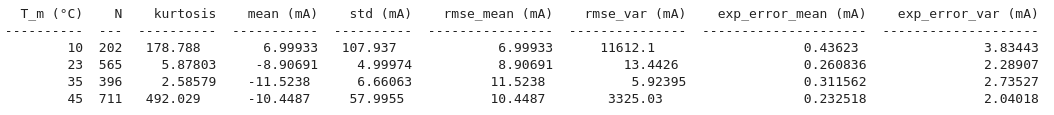
\includegraphics[width=\linewidth]{Images/error_table.png}
        \captionof{table}{Distribution of measurement errors}
        \label{tab:1}
    \end{center}
\end{figure*}

\begin{center}
    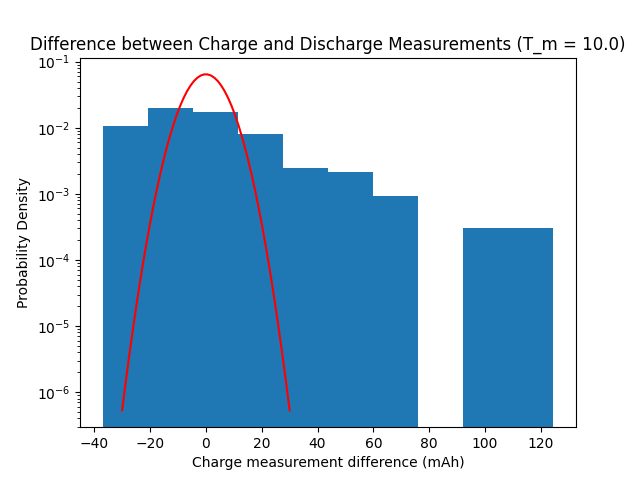
\includegraphics[width=0.9\linewidth]{Images/measurement_error_0.png}
    \captionof{figure}{Measurement Noise PDF for T=10°C}
    \label{fig:meas-noise0}
\end{center}

\begin{center}
    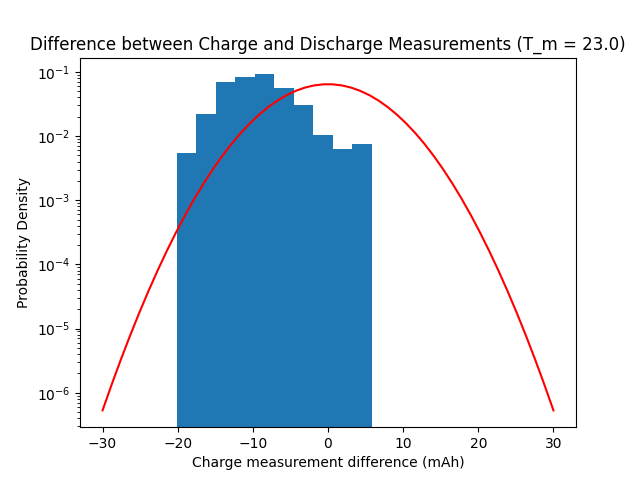
\includegraphics[width=0.9\linewidth]{Images/measurement_error_1.png}
    \captionof{figure}{Measurement Noise PDF for T=23°C}
    \label{fig:meas-noise1}
\end{center}

\begin{center}
    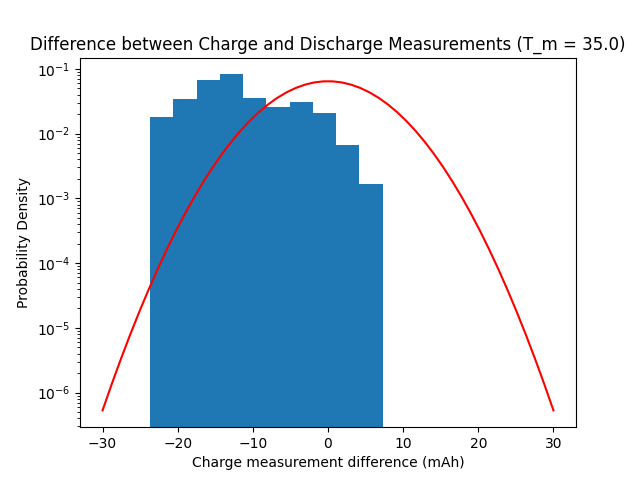
\includegraphics[width=0.9\linewidth]{Images/measurement_error_2.png}
    \captionof{figure}{Measurement Noise PDF for T=35°C}
    \label{fig:meas-noise2}
\end{center}

\begin{center}
    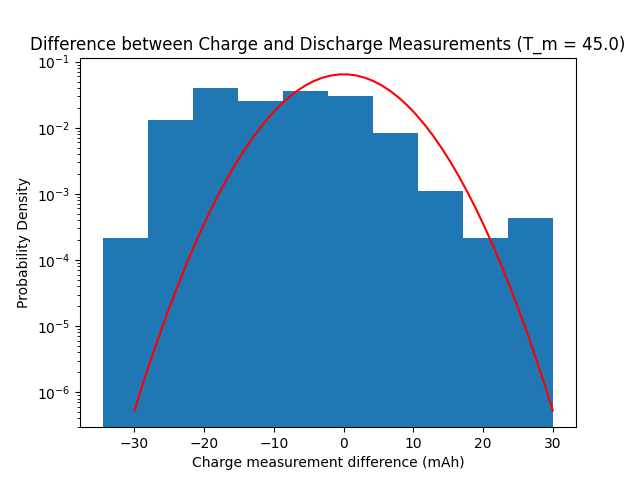
\includegraphics[width=0.9\linewidth]{Images/measurement_error_3.png}
    \captionof{figure}{Measurement Noise PDF for T=45°C}
    \label{fig:meas-noise3}
\end{center}

\subsection{Cell-to-Cell Variation}

Figure \ref{fig:cell-to-cell-var} shows a histogram of the
measured cell-to-cell variance. The computed cell-to-cell
variance across all operating conditions, $\sigma_c$ is found to
be 457 mAh$^2$.

\begin{center}
    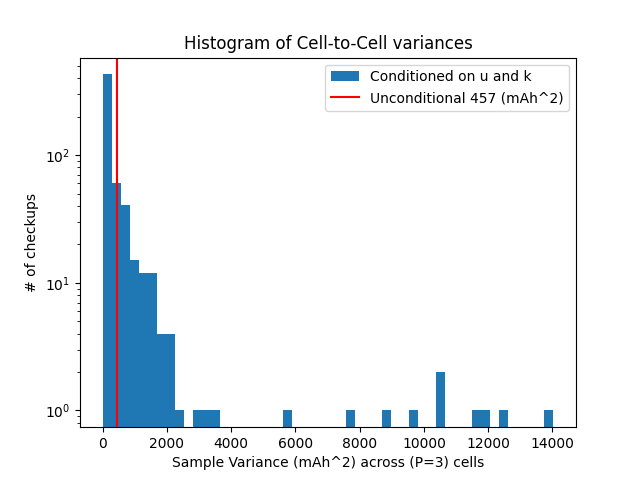
\includegraphics[width=0.9\linewidth]{Images/cond_cell_to_cell_var.png}
    \captionof{figure}{Variance between Cells}
    \label{fig:cell-to-cell-var}
\end{center}


\subsection{Gaussian Process Regression}


Plots for the regression with 3 features ($N=3$) are displayed.
Results for a few representative operating conditions are shown
in Figures \ref{fig:gp-low-var}-\ref{fig:gp-spur-var}.

The different colored dots indicate the three different cells
tested under those conditions.

The blue shaded region shows the $\pm$2 std range of the
GP prediction, while the solid blue line shows the prediction mean.

\begin{center}
    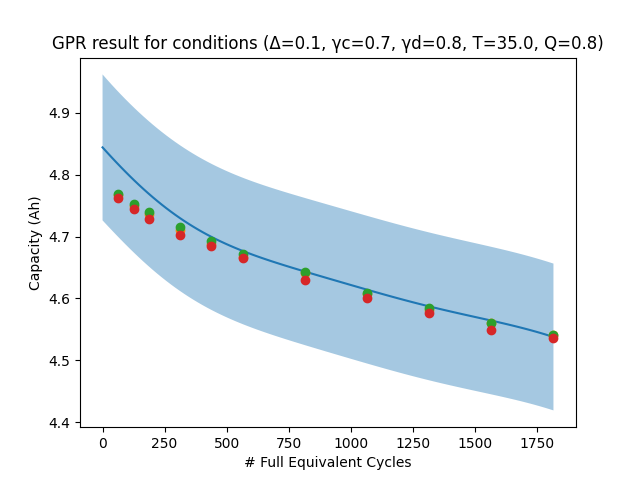
\includegraphics[width=0.9\linewidth]{Images/gp_low_var.png}
    \captionof{figure}{GPR result for a low-cell-to-cell variance cycle}
    \label{fig:gp-low-var}
\end{center}
\begin{center}
    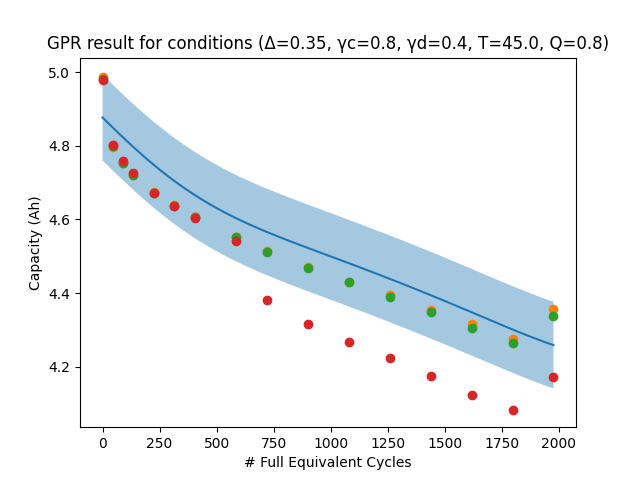
\includegraphics[width=0.9\linewidth]{Images/gp_strange_drop.png}
    \captionof{figure}{GPR result with greatest cell-to-cell variance}
    \label{fig:gp-high-var}
\end{center}
\begin{center}
    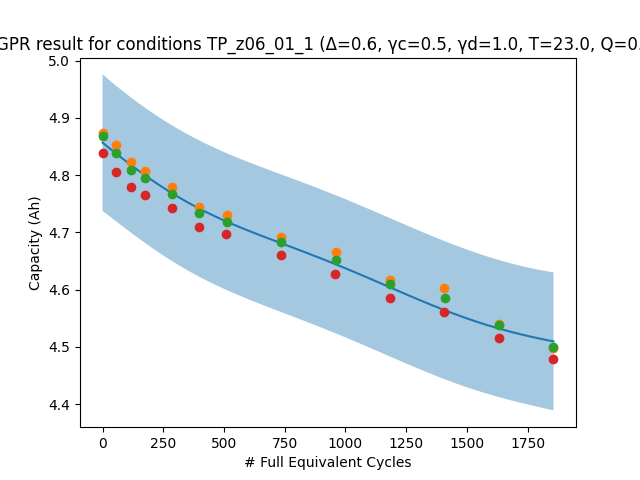
\includegraphics[width=0.9\linewidth]{Images/gp_typ.png}
    \captionof{figure}{Typical GPR result}
    \label{fig:gp-mid-var}
\end{center}

\begin{center}
    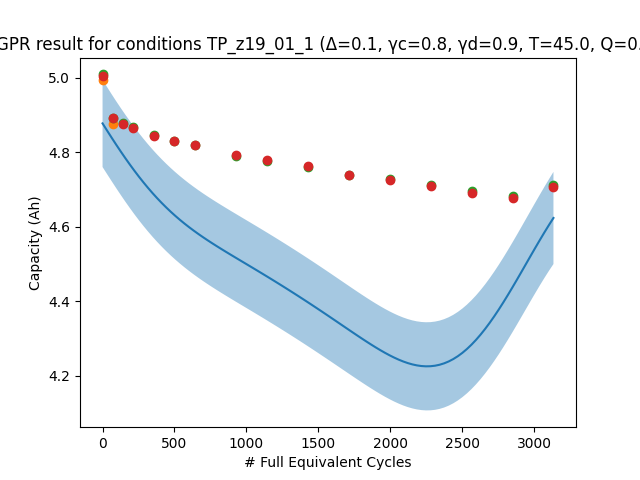
\includegraphics[width=0.9\linewidth]{Images/gp_spurious.png}
    \captionof{figure}{Spurious GPR result}
    \label{fig:gp-spur-var}
\end{center}

The optimized hyperparameters $\theta$ are shown in table \ref{table:hyp}.

\begin{center}
\begin{tabular}{||c | c c c c||} 
 \hline
  & Optimal & Initial & Lower Bound & Upper Bound \\ [0.5ex] 
 \hline\hline
 $\sigma_c$ & 0.1 &  0.1 & 1e-4 & 0.1 \\ 
 \hline
 $\ell_T$ & 13.5 & 10 & 5 & 25 \\
 \hline
 $\ell_{\gamma_c}$ & 0.116 & 0.1 & 1e-3 & 0.2 \\
 \hline
 $\ell_{k}$ & 755.8 & 1000 & 500 & 3000 \\
 \hline
\end{tabular}
\label{table:hyp}
\captionof{table}{Hyperparameter Optimization Results}
\end{center}

The error distribution is shown below:
\begin{center}
    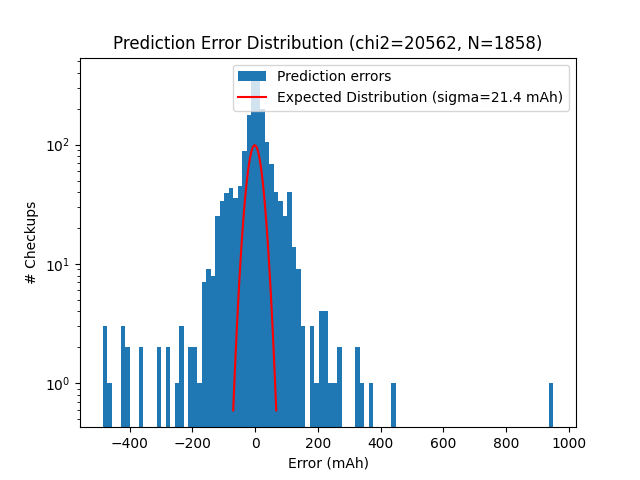
\includegraphics[width=0.9\linewidth]{Images/error_dist.png}
    \captionof{figure}{Distribution of errors}
    \label{fig:error-dist}
\end{center}

% 1.00000000e-01, 1.16044418e-01, 1.34761254e+01, 7.55862929e+02


%         ("gamma_ch", 0.1, [1e-3, 0.2]),
%         ("T", 10, [5, 25]),
%         # ("T_m", 10,
%         ("k", 1000, [500, 3000])



\section{Discussion}

\subsection{Capacity Measurement Noise}

The experimental error in the variance is higher than
the expected variance, which implies that there are other forms of 
error impacting our results. In particular for measurement
temperatures $\hat{T} = 10,45$ there are some major outliers
that are affecting results from table \ref{tab:1}. These have been
removed from the histograms. 

\subsection{Cell-to-cell Variation}

As seen in the historam of figure \ref{fig:cell-to-cell-var},
there are quite a few outlying results. Figure \ref{fig:gp-high-var}
shows the GPR fit for one of those high-variance cases.
To the eye, these measurements appear obviously incorrect. The red-line
has a large step downwards around cycle 750. Cross-referencing with
the original paper: sure enough, these are results from the
test "TP\_z17\_03\_13\_exCU" when the lab experienced a blackout.

We expect that a number of the outlying samples are a result
of this type of experimental error.

It is possible that the unconditional variance of 457 mAh$^2$
was computed incorrectly as there were a number of challenges
with handling nans as well as the inconsistent numbers of checkups
between different cells.


\subsection{Gaussian Process Regression}

From the plots of the fit shown and the error distribution, we see
that for a majority the prediction mean is at least reasonably
close to the observations. It is interesting to note that there
is a smoothing with respect to the number of cycles, particularly
in figure \ref{fig:gp-high-var}.

The $\chi^2$ error is significantly higher than expected, likely
a result of a number of fits such as \ref{fig:gp-spur-var}
which are for some reason entirely incorrect.

The author was hoping to generate a plot showing 2d heat map
across the other axes of the feature vector. However, due
to the sparse nature of the dataset being fit, it is difficult
to find fixed parameters across the other dimensions which
contain enough datapoint for the plot to be meaningful.


\section{Conclusion}

Gaussian Process Regression is a useful and general tool to
estimate noisy processes over a general space
(whether that space is spatial or more generally corresponds to some
features).

We performed statistical analysis to determining the various sources
of noise within a comprehensive and diverse LiB aging dataset.
While it is challenging to visualize such a dataset over all
of its axes simulataneously, GPR can algorithmically accomodate
by estimating higher uncertainty in these regions.

Quite a bit of noise is introduced in the dataset related
to experimental error. A more methodical way of filtering
such error from the various other sources of noise may be fruitful.

There remains more work to do in identifying the sources of the
number of dubious artifacts contained in both the dataset
and the regression model, but this project lays a foundation 
in that direction.








\bibliography{SE_project}
\bibliographystyle{ieeetr}

\vspace{12pt}

\end{document}
